\documentclass[11pt]{article}
\usepackage[margin=1in]{geometry}
\usepackage[T1]{fontenc}
\usepackage[utf8]{inputenc}
\usepackage{lmodern}
\usepackage{hyperref}
\usepackage{xcolor}
\usepackage{enumitem}
\usepackage{amsmath}
\usepackage{booktabs}
\usepackage{array}
\usepackage{longtable}
\usepackage{tabularx}
\usepackage{graphicx}
\usepackage{tikz}
\usetikzlibrary{arrows.meta,positioning,shapes.geometric,fit}
\usepackage{fancyhdr}
\pagestyle{fancy}
\fancyhf{}
\rhead{ROBERT Agent Project Plan}
\lhead{Draft for Overleaf}
\cfoot{\thepage}

\hypersetup{
  colorlinks=true,
  linkcolor=blue,
  urlcolor=blue,
  pdftitle={ROBERT Agent Project Plan},
  pdfauthor={Chris Collison}
}

\setlist[itemize]{leftmargin=1.4em}
\setlist[enumerate]{leftmargin=1.8em}

\title{Project Plan: Building a ROBERT Companion Agent}
\author{Working Draft for Discussion and Iteration}
\date{\today}

\begin{document}
\maketitle

\section{Project Goal}
The goal of this project is to design and prototype a companion agent for \textbf{ROBERT} that helps chemists understand, diagnose, and improve their model results. The first and most important capability is narrow and concrete:

\begin{quote}
\textit{Given the output of a ROBERT run, answer the question: ``Why did I get this ROBERT score?''}
\end{quote}

The central design principle is to start small, solve one question well, and scale only after the reasoning workflow is understood.

\section{Why This Is the Right Starting Point}
Users can often run ROBERT successfully, but they struggle to interpret the results. In practice, the most common question is not how to execute the software, but what the score means and what to do next. This makes score interpretation an ideal anchor problem because it forces the system to connect:

\begin{itemize}
    \item dataset size and quality,
    \item feature curation decisions,
    \item split strategy,
    \item cross-validation stability,
    \item verification tests,
    \item outliers,
    \item feature importance and chemical plausibility.
\end{itemize}

If an agent can answer this question well, it will already be useful. More advanced capabilities (descriptor suggestions, scaffold splitting, specialized chemistry heuristics, UI integration, persistent threads, and hosted deployment) can come later.

\section{High-Level Strategy}
The recommended strategy is to build the system in four layers:

\begin{enumerate}
    \item \textbf{Reasoning layer:} define exactly how a human expert explains a ROBERT score.
    \item \textbf{File mapping layer:} identify which ROBERT output files contain the needed evidence.
    \item \textbf{Prototype layer:} implement a simple Python program that reads the outputs and produces a structured explanation.
    \item \textbf{LLM layer:} connect the structured explanation to an OpenAI model so the results can be explained naturally to the user.
\end{enumerate}

\section{Core Principle}
The LLM should \textbf{not} be the first source of reasoning. Instead:

\begin{itemize}
    \item deterministic rules and extracted evidence should identify the likely reasons for the score,
    \item the LLM should translate those findings into a coherent chemistry-facing explanation,
    \item the system should remain auditable.
\end{itemize}

\section{Current Approach (Living Snapshot)}
This section is updated regularly to reflect the current implementation approach.
It is client-facing and intentionally concise. The source-of-truth execution logs
are maintained in the project markdown trackers.

\subsection*{Verified Technical Anchors}
\begin{itemize}
    \item \textbf{ROBERT score computation:} implemented in \texttt{robert/report\_utils.py} in \texttt{calc\_score}, with contributions from \texttt{get\_predict\_scores} and \texttt{get\_verify\_scores}.
    \item \textbf{PDF generation:} orchestrated in \texttt{robert/report.py}; PDF writing performed by \texttt{make\_report} and \texttt{make\_pdf}.
    \item \textbf{Primary evidence files:} \texttt{PREDICT/PREDICT\_data.dat} and \texttt{VERIFY/VERIFY\_data.dat}.
    \item \textbf{Supplementary provenance files:} \texttt{CURATE/CURATE\_data.dat}, \texttt{GENERATE/GENERATE\_data.dat}, and model parameter CSV files in \texttt{GENERATE/Best\_model}.
\end{itemize}

\subsection*{Current Working Policy}
\begin{itemize}
    \item Work in small, reviewable increments.
    \item Preserve proposed plans in a dedicated section before execution.
    \item Keep implementation read-only with respect to existing ROBERT core code.
\end{itemize}

\subsection*{Progress Reporting Convention}
\begin{itemize}
    \item \textbf{Source of truth (operational):} TODO and completed-task trackers.
    \item \textbf{Client-facing summary:} this \texttt{.tex} document.
\end{itemize}

\section{Project Flowchart}
\begin{center}
\resizebox{\textwidth}{!}{
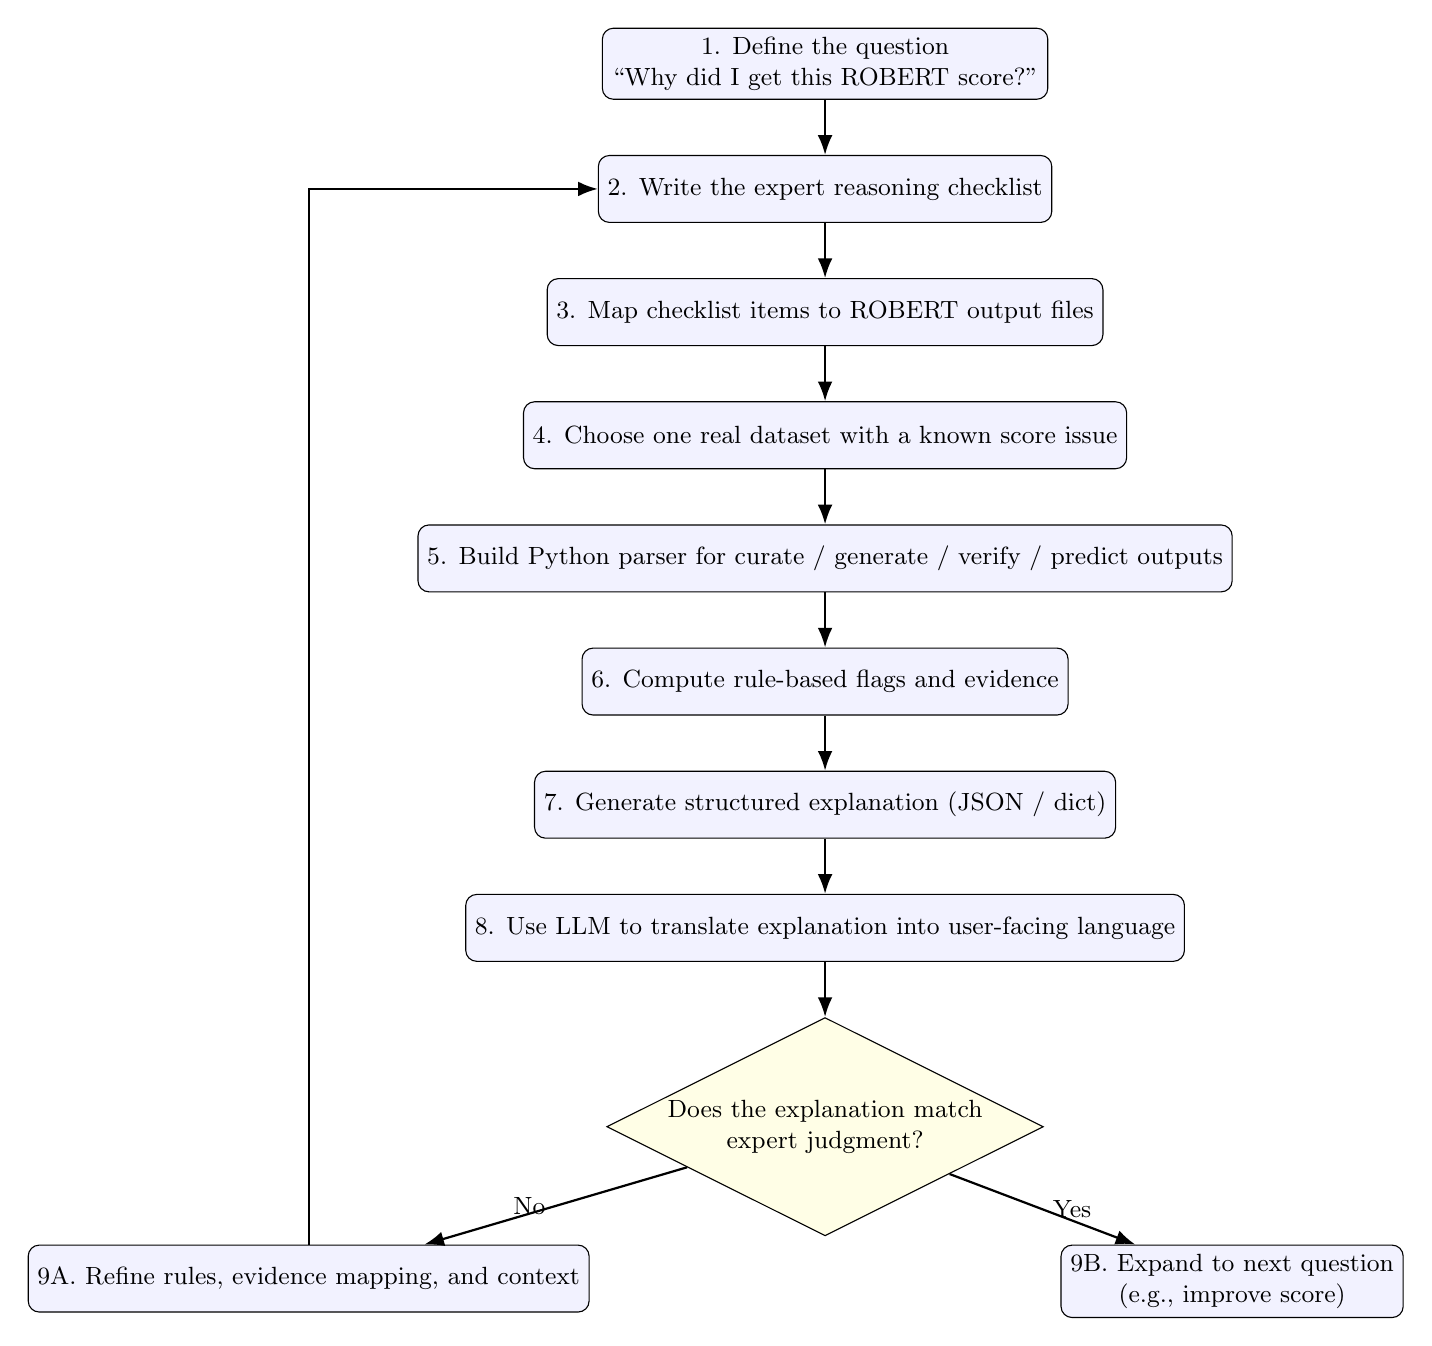
\begin{tikzpicture}[
    node distance=0.7cm and 1.0cm,
    box/.style={draw, rounded corners, align=center, minimum width=3.2cm, minimum height=0.85cm, fill=blue!5},
    decision/.style={draw, diamond, aspect=2, align=center, fill=yellow!10, inner sep=1pt},
    arrow/.style={-{Latex[length=2.5mm]}, thick},
    font=\small
]

\node[box] (r1) {1. Define the question\\``Why did I get this ROBERT score?''};
\node[box, below=of r1] (r2) {2. Write the expert reasoning checklist};
\node[box, below=of r2] (r3) {3. Map checklist items to ROBERT output files};
\node[box, below=of r3] (r4) {4. Choose one real dataset with a known score issue};
\node[box, below=of r4] (r5) {5. Build Python parser for curate / generate / verify / predict outputs};
\node[box, below=of r5] (r6) {6. Compute rule-based flags and evidence};
\node[box, below=of r6] (r7) {7. Generate structured explanation (JSON / dict)};
\node[box, below=of r7] (r8) {8. Use LLM to translate explanation into user-facing language};
\node[decision, below=of r8] (d1) {Does the explanation match\\expert judgment?};

\node[box, below left=0.8cm and 1.6cm of d1] (r9a) {9A. Refine rules, evidence mapping, and context};
\node[box, below right=0.8cm and 1.6cm of d1] (r9b) {9B. Expand to next question\\(e.g., improve score)};

\draw[arrow] (r1) -- (r2);
\draw[arrow] (r2) -- (r3);
\draw[arrow] (r3) -- (r4);
\draw[arrow] (r4) -- (r5);
\draw[arrow] (r5) -- (r6);
\draw[arrow] (r6) -- (r7);
\draw[arrow] (r7) -- (r8);
\draw[arrow] (r8) -- (d1);
\draw[arrow] (d1) -- node[left]{No} (r9a);
\draw[arrow] (d1) -- node[right]{Yes} (r9b);
\draw[arrow] (r9a.north) |- (r2.west);

\end{tikzpicture}
}
\end{center}

\section{Detailed Step-by-Step Checklist}

\subsection{Phase 1: Define the Reasoning Problem}
\textbf{Objective:} Turn the abstract question into a concrete reasoning framework.

\subsubsection*{Step 1.1 --- Write the exact anchor question}
Write the question exactly as follows and keep it fixed for version 1:

\begin{quote}
\textbf{Why did I get this ROBERT score?}
\end{quote}

This should remain the only supported question in the first prototype.

\subsubsection*{Step 1.2 --- Write what a human expert would inspect}
Create a checklist titled \textit{How a human expert explains a ROBERT score}. Include items such as:

\begin{enumerate}
    \item How many rows are in the dataset?
    \item How many descriptors existed before and after curation?
    \item What split strategy was used?
    \item What is the difference between CV and test performance?
    \item Did any verification tests fail or look suspicious?
    \item Are there strong outliers?
    \item Are the important features chemically meaningful?
    \item Is the target difficult because of system complexity, data sparsity, or representation mismatch?
\end{enumerate}

\subsubsection*{Step 1.3 --- Convert the checklist into categories}
Group the checklist into categories. One possible grouping is:

\begin{itemize}
    \item \textbf{Data adequacy}
    \item \textbf{Feature curation and pruning}
    \item \textbf{Model stability}
    \item \textbf{Verification logic}
    \item \textbf{Outliers and error structure}
    \item \textbf{Chemical plausibility}
\end{itemize}

\subsection{Phase 2: Map Reasoning to ROBERT Outputs}
\textbf{Objective:} Identify where the evidence comes from.

\subsubsection*{Step 2.1 --- Build a file-evidence table}
Make a table like Table~\ref{tab:evidence} and refine it as the repo is explored.

This should expand into a full ROBERT report extraction checklist so the companion agent
can surface warnings, caveats, score components, VERIFY results, PREDICT metrics,
outliers, feature importance, curation details, and report or PDF evidence artifacts.
Each surfaced item should link back to a concrete evidence source such as
\texttt{run\_context.json}, \texttt{diagnosis.json}, \texttt{PREDICT\_data.dat},
\texttt{VERIFY\_data.dat}, \texttt{CURATE\_data.dat}, \texttt{GENERATE\_data.dat},
model parameter CSV files, or report artifacts.

\begin{longtable}{p{0.29\textwidth} p{0.27\textwidth} p{0.34\textwidth}}
\caption{Evidence mapping for score interpretation.}\label{tab:evidence}\\
\toprule
\textbf{Reasoning question} & \textbf{Likely ROBERT source} & \textbf{What to extract} \\
\midrule
\endfirsthead
\toprule
\textbf{Reasoning question} & \textbf{Likely ROBERT source} & \textbf{What to extract} \\
\midrule
\endhead
Dataset size & Curated CSV / input summary & Number of rows, target range, missingness \\
Feature pruning & \texttt{curate/} outputs & Feature count before/after pruning, correlated feature removals \\
Split strategy & \texttt{generate/} outputs & Split mode, train/test sizes, fold structure \\
Model quality & \texttt{predict/} outputs & Score, R$^2$, MAE, RMSE, CV vs test gap \\
Verification checks & \texttt{verify/} outputs & y-mean, y-shuffle, onehot outcomes \\
Outlier burden & \texttt{predict/} outputs & Number and severity of outliers \\
Feature meaning & SHAP / PFI outputs & Top ranked descriptors and contribution direction \\
\bottomrule
\end{longtable}

\subsubsection*{Step 2.2 --- Inspect how the PDF is generated}
Locate the code that builds the PDF report and identify:

\begin{itemize}
    \item which files it reads,
    \item how it calculates the ROBERT score,
    \item which intermediate statistics are needed to justify the final score.
\end{itemize}

This is critical because the first agent should explain the score \emph{from the same underlying data that the report uses}, not from the PDF itself.

\subsubsection*{Step 2.3 --- Note which files are stable and which are fragile}
Some output files may be safer to parse than others. Keep notes on:

\begin{itemize}
    \item filenames,
    \item formats (CSV, DAT, TXT, JSON if any),
    \item whether they are version-sensitive,
    \item whether they are directly interpretable or need post-processing.
\end{itemize}

\subsection{Phase 3: Collect a Gold-Standard Test Case}
\textbf{Objective:} Work from a real example, not an abstract one.

Alongside the anchor score question, the first interpretation workflow should also answer:

\begin{quote}
\textbf{What did ROBERT do with my data?}
\end{quote}

This means the extracted context should explain how the original CSV becomes the curated
feature set by tracking the original feature count, removed descriptors, retained
descriptors, and the final descriptors used by the selected model. This is especially
important for cases like ``26 data points, 39 features, final model uses 3 descriptors''
where feature reduction may be expected rather than a sign of failure.

\subsubsection*{Step 3.1 --- Obtain one open dataset}
Ask for one open or shareable dataset with:

\begin{itemize}
    \item a moderate or poor ROBERT score,
    \item a known explanation from expert experience,
    \item ideally a repeated or common user question.
\end{itemize}

Examples:
\begin{itemize}
    \item a small catalyst dataset,
    \item a system where descriptor generation fails or is incomplete,
    \item a case where adding atomic descriptors improves the score,
    \item a case where the user misinterprets a score of 4--6.
\end{itemize}

\subsubsection*{Step 3.2 --- Write the human explanation first}
For this test case, manually answer the anchor question yourself in bullet points.

The result should look something like:

\begin{quote}
The score is limited mainly by small dataset size, instability across validation partitions, and descriptor mismatch for a metal-containing system. The model is not necessarily bad, but the confidence should be interpreted cautiously.
\end{quote}

This human explanation becomes the benchmark that the prototype should reproduce.

\subsection{Phase 4: Build the First Prototype in Python}
\textbf{Objective:} Build the smallest working system without UI.

\subsubsection*{Step 4.1 --- Create a folder structure}
Create a clean working directory, for example:

\begin{verbatim}
robert_agent/
  data/
  examples/
  parsers/
  prompts/
  outputs/
  notes/
\end{verbatim}

\subsubsection*{Step 4.2 --- Write a parser for each ROBERT stage}
Write small Python functions such as:

\begin{verbatim}
read_curate_outputs(path)
read_generate_outputs(path)
read_verify_outputs(path)
read_predict_outputs(path)
\end{verbatim}

Each function should return a dictionary with the most relevant values.

\subsubsection*{Step 4.3 --- Combine them into one context object}
Create a single structured dictionary, e.g.:

\begin{verbatim}
run_context = {
  "dataset": {...},
  "curate": {...},
  "generate": {...},
  "verify": {...},
  "predict": {...}
}
\end{verbatim}

This becomes the internal representation of a ROBERT run.

\subsubsection*{Step 4.4 --- Save the context as JSON}
Write the context object to disk as:

\begin{verbatim}
outputs/run_context.json
\end{verbatim}

This file is useful for debugging and later LLM calls.

\subsection{Phase 5: Add Deterministic Diagnostic Rules}
\textbf{Objective:} Produce evidence-based flags before introducing the LLM.

\subsubsection*{Step 5.1 --- Write simple score-diagnosis rules}
Implement rules such as:

\begin{verbatim}
if n_rows < 50:
    add_flag("Small dataset; score may be limited by sample size")

if abs(cv_metric - test_metric) > threshold:
    add_flag("Large CV/test gap; possible overfitting or unstable split")

if verify_y_shuffle_failed:
    add_flag("Signal may be weak or partly spurious")

if outlier_count > 0:
    add_flag("Outliers may be pulling the score down")
\end{verbatim}

These should not be viewed as final chemistry logic, only a starting framework.

\subsubsection*{Step 5.2 --- Add chemistry-sensitive heuristics later}
Once the first version works, add domain-aware heuristics such as:

\begin{itemize}
    \item metal-containing systems with missing atomic descriptors,
    \item repeated scaffolds that may inflate performance,
    \item regression problems that may be better framed as classification,
    \item descriptor sets that are too homogeneous to be useful.
\end{itemize}

\subsection{Phase 6: Connect the LLM}
\textbf{Objective:} Turn structured evidence into a useful explanation.

\subsubsection*{Step 6.1 --- Define the LLM's role carefully}
The LLM should:

\begin{itemize}
    \item read the structured context,
    \item summarize the likely reasons for the score,
    \item explain them in chemistry-friendly, jargon-free language,
    \item suggest one to three next actions.
\end{itemize}

The LLM should \textbf{not} be responsible for discovering all reasoning from scratch.
It should translate extracted evidence, not invent reasoning, thresholds, or score logic.
When machine-learning terms are necessary, they should be explained in plain language.

\subsubsection*{Step 6.2 --- Standardize the answer structure}
Each response should follow a consistent structure:

\begin{enumerate}
    \item Plain-language summary
    \item Is the model useful?
    \item Main benefits
    \item Caveats and warnings
    \item What ROBERT did with the data
    \item Important descriptors or outliers
    \item Suggested next step
\end{enumerate}

Each response should also suggest one or two useful follow-up questions based on the
current run context.

\subsubsection*{Step 6.3 --- Create a minimal prompt}
A minimal prompt can say:

\begin{quote}
You are assisting a chemist who ran ROBERT. Use only the structured context provided. Explain why the user obtained this ROBERT score, identify the most likely limiting factors, explain what ROBERT did with the user's data, and recommend up to three concrete next steps. Avoid unexplained machine-learning jargon. Do not invent file contents, descriptor meanings, or score logic that are not present in the provided context.
\end{quote}

\subsubsection*{Step 6.4 --- Add starter questions in the UI}
The UI should expose clickable starter questions such as:

\begin{itemize}
    \item Why did I get this ROBERT score?
    \item Is this model reliable enough to use?
    \item What did ROBERT remove from my dataset?
    \item Which descriptors matter most?
    \item Are there warnings I should pay attention to?
    \item What should I try next?
    \item Can you explain this without machine-learning jargon?
    \item What did ROBERT do with my original CSV?
\end{itemize}

\subsubsection*{Step 6.5 --- Save explanations as text}
Save the model output to:

\begin{verbatim}
outputs/score_explanation.txt
\end{verbatim}

Later, this can become part of an interactive system.

\subsection{Phase 7: Evaluate Against Expert Judgment}
\textbf{Objective:} Determine whether the prototype is useful.

\subsubsection*{Step 7.1 --- Compare prototype vs expert explanation}
For the chosen test dataset, compare:

\begin{itemize}
    \item the human explanation,
    \item the rule-based flags,
    \item the LLM-generated explanation.
\end{itemize}

Assess whether the generated explanation:

\begin{itemize}
    \item identifies the right root causes,
    \item avoids hallucinations,
    \item suggests sensible next steps,
    \item uses chemistry language appropriately.
\end{itemize}

\subsubsection*{Step 7.2 --- Keep a simple evaluation rubric}
Use a 1--5 score for each of these:

\begin{enumerate}
    \item Correctness
    \item Relevance
    \item Chemical usefulness
    \item Actionability
    \item Faithfulness to ROBERT outputs
\end{enumerate}

\subsection{Phase 8: Decide How to Scale}
\textbf{Objective:} Only scale after the reasoning works.

Once the Python prototype works, the next levels can be considered:

\begin{enumerate}
    \item \textbf{Standalone local assistant} using Python + API key.
    \item \textbf{Local browser wrapper} using Streamlit or similar.
    \item \textbf{Integrated optional ROBERT add-on} in the GitHub repo.
    \item \textbf{Hosted agent with persistent threads and broader context.}
    \item \textbf{Browser-based ROBERT execution from uploaded CSV} as a separate future workflow.
    \item \textbf{Educational mode} to teach the user what ROBERT is doing step by step.
    \item \textbf{Guided report walkthrough} that explains one report section at a time.
    \item \textbf{Simplified notebooks} where each section begins with a plain-language explanation followed by one simple function call.
\end{enumerate}

The key is that the reasoning engine should remain the same across these stages.

\section{Suggested Immediate To-Do List}
If this project is started now, the first concrete tasks should be:

\begin{enumerate}
    \item Write the one-page \textit{expert score reasoning checklist}.
    \item Inspect the ROBERT code that generates the report and the score.
    \item Build the evidence mapping table between reasoning questions and ROBERT files.
    \item Obtain one open dataset with a known score issue.
    \item Write the first Python parser for one example run.
    \item Generate the first \texttt{run\_context.json}.
    \item Write three to five deterministic diagnostic rules.
    \item Test whether the explanation matches expert judgment.
\end{enumerate}

\section{What Additional Inputs May Be Needed}
The following may become useful during iteration:

\begin{itemize}
    \item the ROBERT paper,
    \item the code that generates the PDF report,
    \item the code or files involved in ROBERT score computation,
    \item a sample of the \texttt{curate}, \texttt{generate}, \texttt{verify}, and \texttt{predict} folders from one run,
    \item one or more open datasets with known interpretation challenges,
    \item later, a short FAQ or repeated user question log from the ROBERT team.
\end{itemize}

\section{Recommended Scope Control}
To avoid losing focus, the following should \textbf{not} be part of version 1:

\begin{itemize}
    \item rebuilding ROBERT or duplicating its machine-learning logic,
    \item modifying code under \texttt{robert/} without explicit approval,
    \item full chatbot UI,
    \item hosted service,
    \item fine-tuning a custom model,
    \item scaffold splitting implementation,
    \item descriptor recommendation engine,
    \item automatic rerunning of ROBERT,
    \item learning from all prior conversations.
\end{itemize}

These are all good long-term directions, but they should follow a successful proof of concept.

\section{Summary}
The most effective way to start this project is to begin with one narrow, high-value question and build a transparent reasoning pipeline around it. The first version should not try to be a full agent. It should instead be a structured Python prototype that reads the core ROBERT outputs, diagnoses why a score was obtained, and explains the result clearly. Once this works for one real dataset and one common user question, the system can be scaled into a more capable and polished assistant.

\end{document}
